\section{Experimental Details}
\label{app:xp_details}

\subsection{Models, training and evaluation}
\label{app:setup}

\paragraph{Models.} All frozen models are base (pretrained) checkpoints loaded in 4-bit NF4 with double quantization (bitsandbytes), except Mistral-7B-Instruct-v0.3 and Gemma-2-9B-it, which are instruction-tuned and prompted through their chat template. We use Qwen2.5 at 0.5B, 1.5B, 3B, 7B, 14B and 32B parameters, Qwen3-8B-Base, Llama-3.1-8B, Mistral-7B-v0.1, Mistral-7B-Instruct-v0.3 and Gemma-2-9B-it. Most experiments use Qwen2.5-7B.

\paragraph{Adapters and training.} Unless stated otherwise, adapters are LoRA of rank 16 with scale $\alpha = 32$ ($\alpha/r = 2$) and no dropout, on the attention and MLP projections of every layer (q, k, v, o, gate, up and down). We train with AdamW at learning rate $2\times10^{-4}$, $\beta = (0.9, 0.95)$, no weight decay, 3\% linear warmup, gradient clipping at 1.0, effective batch size 16 (micro-batches of 4) and maximum sequence length 1,024 tokens, with the loss on the whole response. The corruption experiments of Section~\ref{sec:recovery} train for one epoch on 32,000 MetaMathQA rows (2,000 updates), and evaluate the validation loss every 200 updates. The adapters of Figure~\ref{fig:families} and of the 14B and 32B studies keep the checkpoint with the lowest validation loss; the Qwen2.5-7B window-search adapters keep the final one. Seeds are 11, 22 and 33 where three are reported, and 11 otherwise.

\paragraph{Evaluation.} Decoding is greedy. GSM8K-style tasks allow 512 new tokens and are scored by exact match of the final answer; MATH-500 allows 1,024 tokens and is checked with Math-Verify; multiple-choice probes ask for a letter within 32 tokens. GSM8K uses all 1,319 test problems where stated and a fixed subset of 500 otherwise. Intervals are 95\% paired bootstrap intervals over questions (2,000 to 10,000 draws), clustered by template for GSM-Symbolic.

\paragraph{Selecting spectral filters.} For the window searches of Section~\ref{sec:recovery}, the corrupted update is decomposed by SVD into its 16 singular directions. Each candidate keeps a set of directions at full precision or codes them. Candidates are scored on 128 MetaMathQA rows reserved from training (every seed problem of the training slice is excluded), the finalists are re-scored on 128 further reserved rows, and only the selected filter is scored on the test sets.

\paragraph{Compute.} Training and evaluation ran on single NVIDIA H100 or A100 GPUs (80\,GB) of the Jean-Zay cluster (IDRIS).

\subsection{Corruptions}
\label{app:corruptions}

\begin{table}[h]
\caption{Corruptions used, with the number of configurations that use each.}
\label{tab:corruptions}
\centering
\small
\begin{tabular}{p{0.3\linewidth}p{0.52\linewidth}r}
\toprule
 & corruption & configs \\
\midrule
rationale permuted & each worked explanation/CoT moved to a different problem; question and answer line kept & 19 \\
response mismatched & the whole response dealt to a different item, for tasks without an answer line & 10 \\
rationale steps shuffled & steps of the explanation reordered; steps, arithmetic and answer kept & 2 \\
arithmetic corrupted & half the computed results moved by up to a third, and the answer follows the wrong chain & 2 \\
labels scrambled / flipped & each multiple-choice letter, or short text label, moved to another of its choices & 2 + 2 \\
\bottomrule
\end{tabular}
\end{table}


\subsection{Codecs and rate accounting}
\label{app:codecs}

Rates are the size of the serialized file, decoding metadata included, divided by the number of scalar values in the uncompressed adapter. The uniform code is a zero-free midrise quantizer fitted per row; the exact-zero control is a midtread quantizer scaled by the row's absolute maximum. LoRAQuant runs in four configurations: 2@0.8, 2@0.9, 3@0.8 and 3@0.9. Below one bit per value we remove paired rank directions before coding. Table~\ref{tab:codecs} lists the rates each code realises.

\begin{table}[h]
\caption{Realised rate and retained GSM8K gain per codec (Mistral-7B, 3 seeds, raw gain 61.5 points).}
\label{tab:codecs}
\centering
\small
\begin{tabular}{lrrr}
\toprule
codec & bits / value & gain kept (\%) & relative RMSE \\
\midrule
midtread, 2 levels (exact zero) & 0.63 & 61.1 & 0.881 \\
adaptive, may drop rows, target 1 & 0.98 & 2.6 & 0.537 \\
uniform zero-free, 1 bit & 1.02 & 85.7 & 0.563 \\
adaptive, keeps rows, target 1.1 & 1.03 & 85.9 & 0.561 \\
LoRAQuant 2@0.8 & 1.59 & 95.4 & -- \\
uniform zero-free, 2 bits & 1.97 & 98.6 & 0.314 \\
LoRAQuant 3@0.9 & 2.69 & 99.1 & -- \\
uniform zero-free, 3 bits & 2.84 & 99.8 & 0.184 \\
uniform zero-free, 4 bits & 3.39 & 100.7 & 0.112 \\
uniform zero-free, 8 bits & 7.28 & 100.1 & 0.008 \\
\bottomrule
\end{tabular}
\end{table}

The compressed adapters of Figure~\ref{fig:families} use the uniform code below one bit: half of the rank directions are removed and the rest are coded at 1 bit, 0.52 bits per value overall and 2.63 to 2.74\,MB depending on the model. The rank-1 codes of Figure~\ref{fig:rank-bits} and Table~\ref{tab:scale} keep the leading singular direction of the update; a rank-1 adapter at 1 bit is a 0.40\,MB file for Qwen2.5-7B.

\subsection{Candidates for the behavioral rate}
\label{app:negative}

\begin{figure}[h]
\centering
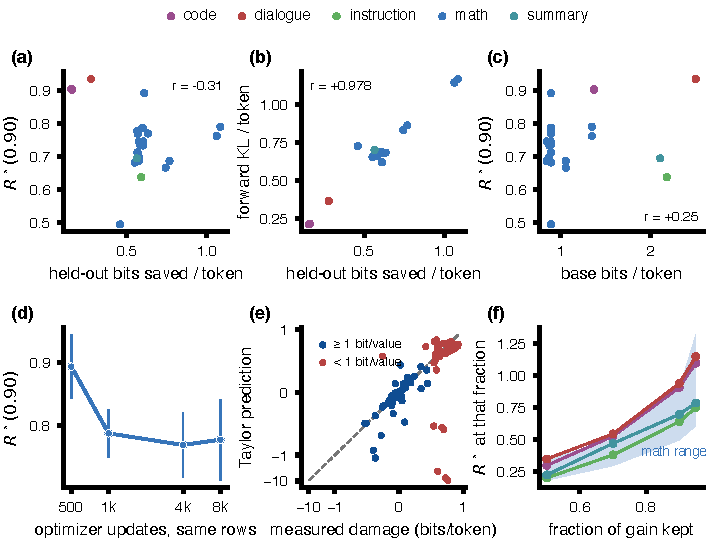
\includegraphics[width=\linewidth]{figures/A2_negative_battery.pdf}
\caption{Candidates for predictors of $R^\star(0.90)$, one point per arm (seed means; 24 arms, Mistral-7B). (a) Held-out bits saved: $r=-0.31$. (b) Forward KL tracks bits saved at $r=+0.978$, so it is not a second measurement. (c) Base bits per token on the corpus: $r=+0.25$. (d) Sixteen times the optimizer updates on the same rows lowers $R^\star$; bars are seed s.d. (e) Second-order Taylor prediction of the damage against measured damage, symmetric log axes: close above one bit per value, wrong in sign and size below it. (f) $R^\star$ at other retention thresholds: code and dialogue sit at the top of the math range at every threshold.}
\label{fig:a2}
\end{figure}

The audit re-scored 268 cells from 67 arms on four receivers with 46 candidate measures, after six repairs to the measurement pipeline; nothing was retrained. The repairs lower the held-out-receiver error from 0.239 (receiver mean) to 0.152, but the best predictor is text cross-row redundancy, two zlib calls that never look at the model (Figure~\ref{fig:a3}). A measure of the corpus alone assigns one value to a corpus on every receiver, so it cannot produce the corpus--receiver reorderings of Section~\ref{sec:behavior-prediction}.

\begin{figure}[h]
\centering
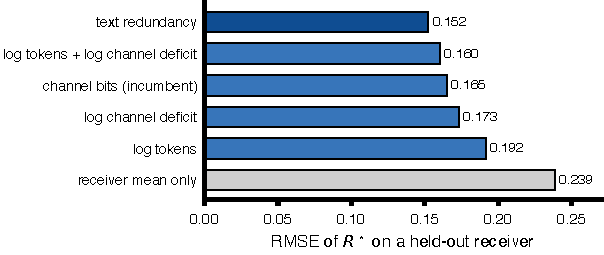
\includegraphics[width=0.66\linewidth]{figures/A3_rate_law_audit.pdf}
\caption{Leave-one-receiver-out RMSE of $R^\star(0.90)$ for the rate-law models, four receivers.}
\label{fig:a3}
\end{figure}

Table~\ref{tab:external} lists every test of a correction statistic on a receiver outside the development pair. Only the locked rows were chosen before seeing that receiver’s \(R^\star\); the rest are shown for completeness.

\begin{table}[h]
\caption{Correction statistics on new receivers. $\rho$: Spearman between measure and $R^\star(0.90)$ over natural corpora (seed means). RMSE: absolute prediction from the development fit, against the base-code-length fit. Gate: $\rho\ge0.70$ and lower RMSE than base code length.}
\label{tab:external}
\centering
\small
\setlength{\tabcolsep}{4pt}
\begin{tabular}{llcrrrr}
\toprule
receiver & measure & locked & corpora & $\rho$ & RMSE & base RMSE \\
\midrule
Llama-3.1-8B & Fisher log-volume & yes & 5 & $-0.10$ & 0.357 & 0.327 \\
Qwen3-8B & Fisher effective rank & yes & 4 & $-0.40$ & 0.408 & 0.306 \\
Qwen2.5-7B, new panel & coherent energy / entropy & yes & 5 & 0.10 & 0.296 & 0.241 \\
\midrule
Llama-3.1-8B & coherent energy / entropy & no & 5 & 0.70 & 0.132 & 0.327 \\
Qwen3-8B & coherent energy / entropy & no & 4 & 0.80 & 0.163 & 0.306 \\
Qwen3-8B & coherent energy & no & 4 & 1.00 & 0.206 & 0.306 \\
Llama-3.1-8B & Fisher log-determinant & no & 5 & $-0.50$ & 0.483 & 0.327 \\
Qwen3-8B & Fisher log-determinant & no & 4 & 0.40 & 0.461 & 0.306 \\
Qwen2.5-7B, new panel & Fisher log-determinant & no & 5 & 0.70 & 0.234 & 0.241 \\
\bottomrule
\end{tabular}
\end{table}

\subsection{Known payload}
\label{app:payload}

Sixteen single-token labels are assigned to (family, item) pairs; 128 of 192 mappings are taught, and only the rule that generates labels changes between conditions, so the number of independent 4-bit draws behind them is known. This separates the information the data carries relative to the base model, the weights installed, and the serialized rate by construction.

\begin{figure}[h]
\centering
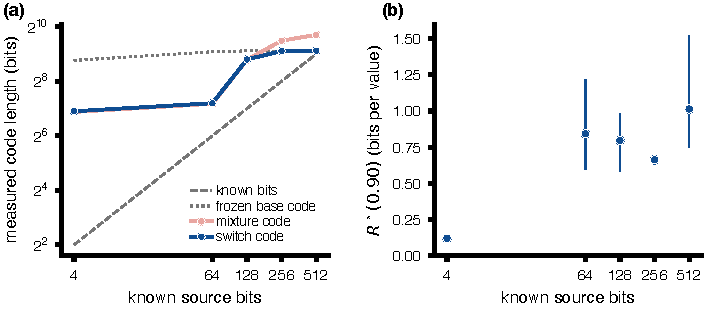
\includegraphics[width=\linewidth]{figures/A4_known_payload.pdf}
\caption{(a) Prequential code length against the known number of source bits. The switch code, which spends one bit per block naming the cheaper of base and adapter, lands within 1.1--3.5$\times$ of the known bits and at most one bit per block above the base code; the plain mixture overshoots the base at 256 and 512 bits. Recall on taught mappings is 1.000 in every cell. (b) $R^\star(0.90)$ does not follow the known information; bars are the seed range. Mistral-7B, 2,048 updates, 3 seeds.}
\label{fig:a4}
\end{figure}

\begin{table}[h]
\caption{GSM8K accuracy (\%) of aligned and permuted adapters under three codes, 3-seed means. Rates: 1.97, 1.50 and 1.02 bits per value.}
\label{tab:a6}
\centering
\small
\begin{tabular}{lrrrrrrrr}
\toprule
 & \multicolumn{4}{c}{aligned} & \multicolumn{4}{c}{permuted} \\
\cmidrule(lr){2-5}\cmidrule(lr){6-9}
model & raw & 2 bits & 1.5 bits & 1 bit & raw & 2 bits & 1.5 bits & 1 bit \\
\midrule
Mistral-7B & 68.9 & 67.3 & 64.2 & 59.3 & 15.7 & 15.3 & 14.3 & 24.2 \\
Qwen2.5-7B & 83.2 & 83.4 & 82.9 & 82.4 & 23.7 & 23.2 & 27.4 & 65.8 \\
Llama-3.1-8B & 73.2 & 72.2 & 70.0 & 65.7 & 19.8 & 19.4 & 17.1 & 34.7 \\
\bottomrule
\end{tabular}
\end{table}

Figure~\ref{fig:r6r7} (Section~\ref{sec:recovery}) repeats the sweep on Qwen2.5-14B and 32B, each with its own corrupted and clean adapters trained as at 7B (rank 16, one epoch on the same 32,000 MetaMathQA rows), except that the checkpoint with the lowest validation loss is kept. At these scales the corrupted adapter falls below base on the search split, so the windows show damage being removed as well as gain added.
% NOTE: Gemma-2-9B-it on NuminaMath-CoT replicates where the damage sits (dropping direction 0 alone restores the base)
% but its selected window does not beat the base on the MATH-500 test (51.2 vs 51.0). Decide whether to report it.
% Mistral-7B-Instruct window search: jobs queued on Jean-Zay, not yet run.

\subsection{All generalization probes}
\label{app:breadth}

Table~\ref{tab:a11} lists the 72 probes behind Figure~\ref{fig:breadth}.

{\small\setlength{\tabcolsep}{4pt}
\begin{longtable}{lrrrrrr}
\caption{All 72 breadth probes. Accuracy on all rows; the last two columns are the held-out half as a fraction of base, where $\dagger$ marks probes the clean adapter hurts on the first half.}\label{tab:a11}\\
\toprule
probe & tier & base & clean & compr. & clean/base & compr./base \\
\midrule\endfirsthead
\toprule probe & tier & base & clean & compr. & clean/base & compr./base \\ \midrule\endhead
\bottomrule\endfoot
gsm8k & 0 & 0.756 & 0.810 & 0.814 & 1.13 & 1.13 \\
asdiv & 1 & 0.885 & 0.925 & 0.902 & 1.07 & 1.03 \\
gsm symbolic & 1 & 0.762 & 0.830 & 0.790 & 1.10 & 1.09 \\
svamp & 1 & 0.790 & 0.847 & 0.890 & 1.08 & 1.15 \\
aqua rat$^\dagger$ & 2 & 0.402 & 0.059 & 0.394 & 0.02 & 1.00 \\
math500$^\dagger$ & 2 & 0.585 & 0.495 & 0.590 & 0.89 & 1.07 \\
MMLU abstract algebra$^\dagger$ & 2 & 0.470 & 0.320 & 0.510 & 0.70 & 1.15 \\
MMLU college mathematics$^\dagger$ & 2 & 0.510 & 0.170 & 0.470 & 0.34 & 0.90 \\
MMLU elementary mathematics$^\dagger$ & 2 & 0.701 & 0.188 & 0.693 & 0.28 & 0.99 \\
MMLU high school mathematics$^\dagger$ & 2 & 0.556 & 0.011 & 0.419 & 0.01 & 0.69 \\
MMLU high school statistics$^\dagger$ & 2 & 0.690 & 0.449 & 0.671 & 0.63 & 0.97 \\
MMLU anatomy & 3 & 0.681 & 0.696 & 0.674 & 1.00 & 0.98 \\
MMLU astronomy$^\dagger$ & 3 & 0.816 & 0.796 & 0.829 & 1.02 & 1.02 \\
MMLU college biology & 3 & 0.840 & 0.806 & 0.847 & 0.92 & 1.00 \\
MMLU college chemistry$^\dagger$ & 3 & 0.480 & 0.390 & 0.460 & 0.81 & 1.04 \\
MMLU college computer science$^\dagger$ & 3 & 0.650 & 0.550 & 0.640 & 0.84 & 1.03 \\
MMLU college physics$^\dagger$ & 3 & 0.451 & 0.284 & 0.431 & 0.48 & 0.91 \\
MMLU computer security & 3 & 0.810 & 0.840 & 0.810 & 1.05 & 1.00 \\
MMLU conceptual physics$^\dagger$ & 3 & 0.711 & 0.634 & 0.719 & 0.86 & 0.99 \\
MMLU electrical engineering$^\dagger$ & 3 & 0.703 & 0.648 & 0.697 & 0.92 & 1.02 \\
MMLU high school biology & 3 & 0.839 & 0.816 & 0.829 & 0.98 & 0.98 \\
MMLU high school chemistry$^\dagger$ & 3 & 0.665 & 0.463 & 0.645 & 0.71 & 0.99 \\
MMLU high school computer science$^\dagger$ & 3 & 0.800 & 0.720 & 0.780 & 0.87 & 0.92 \\
MMLU high school physics$^\dagger$ & 3 & 0.523 & 0.272 & 0.543 & 0.55 & 1.05 \\
MMLU machine learning$^\dagger$ & 3 & 0.491 & 0.411 & 0.509 & 0.73 & 1.08 \\
arc challenge$^\dagger$ & 3 & 0.880 & 0.825 & 0.887 & 0.94 & 1.02 \\
arc easy & 3 & 0.955 & 0.955 & 0.958 & 0.98 & 0.99 \\
openbookqa & 3 & 0.858 & 0.848 & 0.860 & 0.98 & 1.01 \\
qasc & 3 & 0.823 & 0.807 & 0.830 & 0.98 & 1.00 \\
commonsenseqa & 4 & 0.815 & 0.818 & 0.830 & 1.01 & 1.02 \\
hellaswag$^\dagger$ & 4 & 0.855 & 0.710 & 0.845 & 0.76 & 0.99 \\
winogrande & 4 & 0.650 & 0.637 & 0.632 & 0.97 & 0.96 \\
MMLU business ethics & 4 & 0.750 & 0.720 & 0.740 & 0.91 & 0.94 \\
MMLU clinical knowledge & 4 & 0.770 & 0.751 & 0.766 & 0.94 & 1.00 \\
MMLU college medicine$^\dagger$ & 4 & 0.611 & 0.558 & 0.621 & 0.93 & 1.04 \\
MMLU econometrics & 4 & 0.561 & 0.509 & 0.579 & 0.85 & 1.06 \\
MMLU global facts & 4 & 0.440 & 0.470 & 0.410 & 0.96 & 0.96 \\
MMLU high school geography$^\dagger$ & 4 & 0.889 & 0.859 & 0.884 & 1.00 & 1.01 \\
MMLU high school government and politics & 4 & 0.938 & 0.912 & 0.938 & 0.96 & 1.00 \\
MMLU high school macroeconomics & 4 & 0.772 & 0.751 & 0.764 & 0.99 & 0.99 \\
MMLU high school microeconomics & 4 & 0.857 & 0.853 & 0.840 & 1.00 & 0.99 \\
MMLU high school psychology & 4 & 0.873 & 0.870 & 0.873 & 0.98 & 0.99 \\
MMLU human aging & 4 & 0.731 & 0.722 & 0.758 & 1.01 & 1.02 \\
MMLU human sexuality$^\dagger$ & 4 & 0.832 & 0.771 & 0.809 & 0.91 & 0.96 \\
MMLU management & 4 & 0.922 & 0.903 & 0.903 & 0.96 & 0.96 \\
MMLU marketing & 4 & 0.919 & 0.919 & 0.906 & 1.00 & 0.97 \\
MMLU medical genetics & 4 & 0.820 & 0.780 & 0.790 & 0.88 & 0.90 \\
MMLU miscellaneous & 4 & 0.850 & 0.840 & 0.860 & 0.98 & 1.01 \\
MMLU nutrition & 4 & 0.765 & 0.758 & 0.758 & 1.00 & 0.98 \\
MMLU professional accounting$^\dagger$ & 4 & 0.525 & 0.482 & 0.535 & 0.92 & 1.04 \\
MMLU professional medicine & 4 & 0.746 & 0.739 & 0.746 & 0.99 & 1.03 \\
MMLU professional psychology & 4 & 0.735 & 0.715 & 0.740 & 0.98 & 1.03 \\
MMLU public relations$^\dagger$ & 4 & 0.682 & 0.664 & 0.682 & 1.00 & 1.00 \\
MMLU security studies & 4 & 0.763 & 0.771 & 0.771 & 1.01 & 0.99 \\
MMLU sociology & 4 & 0.856 & 0.861 & 0.861 & 1.00 & 1.02 \\
MMLU us foreign policy$^\dagger$ & 4 & 0.940 & 0.870 & 0.900 & 0.96 & 1.00 \\
MMLU virology$^\dagger$ & 4 & 0.554 & 0.512 & 0.530 & 0.93 & 0.98 \\
race high & 4 & 0.882 & 0.875 & 0.882 & 1.00 & 0.99 \\
humaneval & 5 & 0.421 & 0.415 & 0.427 & 0.86 & 1.00 \\
MMLU formal logic$^\dagger$ & 5 & 0.532 & 0.429 & 0.508 & 0.84 & 1.06 \\
MMLU high school european history & 5 & 0.855 & 0.812 & 0.830 & 0.95 & 0.99 \\
MMLU high school us history & 5 & 0.848 & 0.858 & 0.853 & 1.02 & 1.01 \\
MMLU high school world history & 5 & 0.873 & 0.882 & 0.869 & 1.01 & 1.00 \\
MMLU international law & 5 & 0.810 & 0.793 & 0.818 & 0.96 & 1.00 \\
MMLU jurisprudence & 5 & 0.824 & 0.806 & 0.815 & 1.00 & 1.00 \\
MMLU logical fallacies & 5 & 0.828 & 0.804 & 0.828 & 0.96 & 0.99 \\
MMLU moral disputes & 5 & 0.780 & 0.757 & 0.769 & 0.96 & 0.99 \\
MMLU moral scenarios & 5 & 0.292 & 0.395 & 0.237 & 1.26 & 0.76 \\
MMLU philosophy & 5 & 0.740 & 0.720 & 0.746 & 0.98 & 1.04 \\
MMLU prehistory & 5 & 0.809 & 0.784 & 0.796 & 0.98 & 0.97 \\
MMLU professional law & 5 & 0.490 & 0.475 & 0.460 & 0.97 & 0.94 \\
MMLU world religions & 5 & 0.860 & 0.877 & 0.860 & 1.01 & 0.99 \\
\end{longtable}

}
